\subsection{Оптимизатор}

Стадия оптимизации подразумевает несколько обходов по заранее построенному RorenGraph-у.

\subsubsection{Стратегии оптимизации}

В оптимизаторе отдельно выделен интерфейс IStrategy (рис~\ref{fig:strat}), позволяющий коллапсировать оранжевую и красную вершину связанные ребром. Важно, что этот случай подразумевает, что нет другой оранжевой вершины, ребра которой ведут в рассматриваемую красную.

\begin{figure}[h]
    \centering
    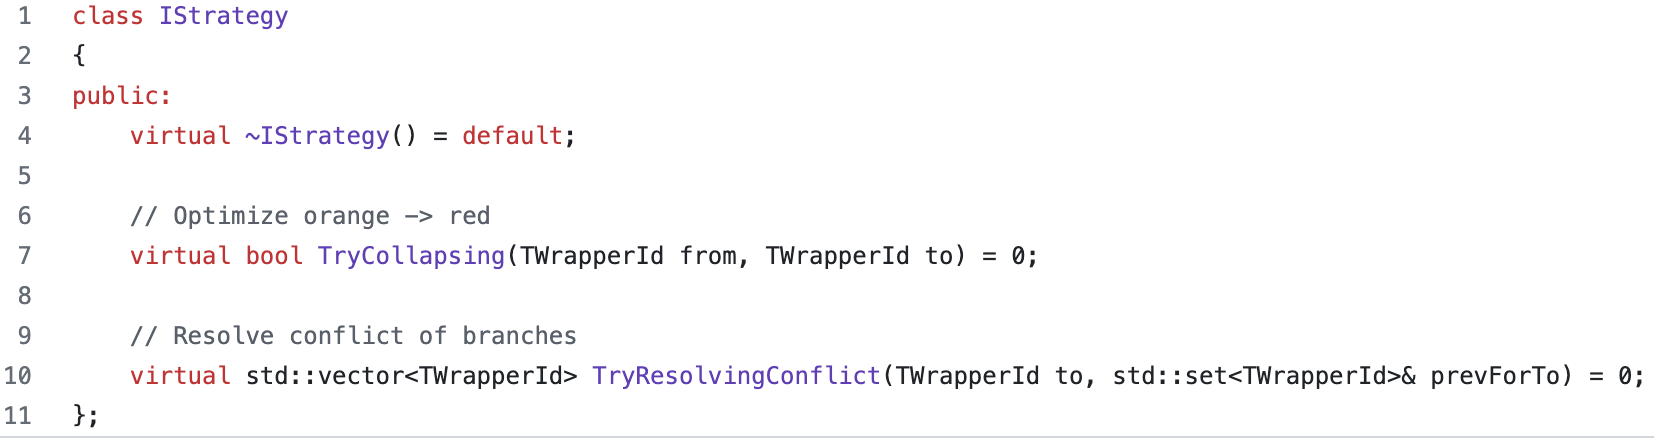
\includegraphics[width=\textwidth]{img/strat.png}
    \caption{Интерфейс стратегии конденсации вершин}
    \label{fig:strat}
\end{figure}

Помимо этого IStrategy позволяет разрешить конфликтную ситуацию, когда есть множество оранжевых вершин, ребра которых ведут в общую красную вершину.

Реализацией данной стратегии может быть стратегия, которая коллапсирует вершины и разрешает конфликты.

Однако это далеко не единственный вариант. Пользователям может понадобится стратегия, которая не сливает параллельные ветви, т.к. это увеличивает latency готовности конкретных таблиц.

Также пользователи могут иметь вычислительно тяжелые операции, требующие большого количества RAM. Так, в случае отдельного запуска операций проблем не будет, но при их слиянии памяти, отведенной на один job, может не хватить.

\newpage
\subsubsection{Предобход для Flatten}

В дизайн Roren заложена концепция, которая позволяет легко описывать в коде графы. Она состоит в том, что у transform-а может быть только один вход. В случае графов с Flatten такой дизайн приведет к тому, что требуется рассматривать несколько слоев transform-ов. Также для упрощения алгоритма мы рассматриваем граф, состоящий из transform-ов, не обращая внимания на коллекции, но сохраняя их.

Для того, чтобы перейти к упрощенному графу требуется сделать предобход, который удалить из графа Flatten, соединяя предыдущие и последующие transform-ы напрямую.
